\documentclass[unicode,10pt]{beamer}
\usepackage{hyperref}
\usepackage{cmap}                
\usepackage[T2A]{fontenc}
\usepackage[utf8]{inputenc}
\usepackage{biblatex}
\usepackage{mathtext}
\usepackage[english, russian]{babel}
\usepackage{commath}
\usepackage{amsfonts}
\usepackage{amssymb}
\usepackage{amsmath}
\usepackage{amsthm}
\usepackage{mathtools}
\usepackage{indentfirst}
\usepackage{geometry}
\usepackage{tikz}
\usepackage{tkz-euclide}
\usetkzobj{all}
\usetikzlibrary{arrows,positioning}
\usetikzlibrary{shapes,snakes}
\usetikzlibrary{shapes.multipart}
\usepackage{graphicx}
\usepackage{epstopdf}
\usepackage{subcaption}
\usepackage{caption}
\usepackage{setspace}
\usepackage{float}
\usepackage{tcolorbox}
\captionsetup{justification=centering}
\DeclareMathOperator*{\argmax}{argmax}
\bibliography{slides.bib}
\mode<presentation>
{
	\usetheme{Warsaw}
	\setbeamercovered{transparent}
	\setbeamertemplate{bibliography item}[text]
}

\newcommand*\diff{\mathop{}\!\mathrm{d}}
\providecommand{\TODO}{\fcolorbox{red}{red}{\large{TODO}}}
\DeclareMathOperator{\upd}{upd}
\DeclareMathOperator{\eol}{eol}
\DeclarePairedDelimiter\ceil{\lceil}{\rceil}
\DeclarePairedDelimiter\floor{\lfloor}{\rfloor}
\providecommand{\err}[1]{$\mathcal{#1}$}
\providecommand{\ev}[1]{$\mathbb{#1}$}
\providecommand{\TODO}[1]{\fcolorbox{red}{red}{\large{FIXME}:#1}}
\setbeamercovered{invisible}
\setbeamertemplate{navigation symbols}{}
\usepackage{physics}

\addtobeamertemplate{navigation symbols}{}{%
    \usebeamerfont{footline}%
    \usebeamercolor[fg]{footline}%
    \hspace{1em}%
    \insertframenumber/\inserttotalframenumber
}

\setlength{\parindent}{1em}
\DeclareMathOperator{\sign}{sign}
\newtheorem{thr}{Теорема}[section]
\addtobeamertemplate{frametitle}{\setlength{\parindent}{0em}}{}
\addtobeamertemplate{block begin}{\setlength{\parindent}{0em}}{\setlength{\parindent}{2em}}
\addtobeamertemplate{block example begin}{\setlength{\parindent}{0em}}{\setlength{\parindent}{2em}}

\makeatletter
\newenvironment{ecases}{%
  \matrix@check\ecases\env@ecases
}{%
  \endarray\right.%
}
\def\env@ecases{%
  \let\@ifnextchar\new@ifnextchar
  \left.
  \def\arraystretch{1.2}%
  \array{@{}l@{\quad}l@{}}%
}


\title{SVM}
\author{Д.\,Корчемкин, В.\,Агеев\,\\622 группа}
\date{\today}

\subject{SVM}

\begin{document}

\begin{frame}
  \maketitle
  	\centering
\end{frame}



\section{SVM}
\begin{frame}{SVM}
	С помощью SVM будет решаться задача классификации

	Входные данные: выборка $\left\{x_i, y_i\right\}_{i=1}^{n}\, x_i \in \mathbb{R}^p, y_i\in\left\{-1,1\right\}$.

	Задача: построить классифицирующее правило 
$$h:\mathbb{R}^p\rightarrow \left\{-1,1\right\}$$
такое, что $y_i\sim h\left(x_i\right)$ в некотором смысле.

\end{frame}


\subsection{Линейно-разделимый случай}
\begin{frame}{Hard-margin SVM}
	Предположим, что данные -- разделимы гиперплоскостью
	$$x^\intercal \beta - \beta_0 = 0; \beta\in\mathbb{R}^p, \beta_0\in\mathbb{R}$$

	Определив величину, пропорциональную расстоянию до гиперплоскости (с знаком)
	$$g\left(x\right)=x^\intercal \beta - \beta_0$$
можно построить классифицирующее правило
	$$h\left(x\right)=\sign\left[g\left(x\right)\right]$$

	Из интуитивных соображений разумно полагать, что наилучшая разделяющая гиперплоскость -- та, которая
расположена дальше всего от представителей каждого из классов.
\end{frame}

\begin{frame}{Hard-margin SVM: margin, decision boundary}
	\begin{figure}
		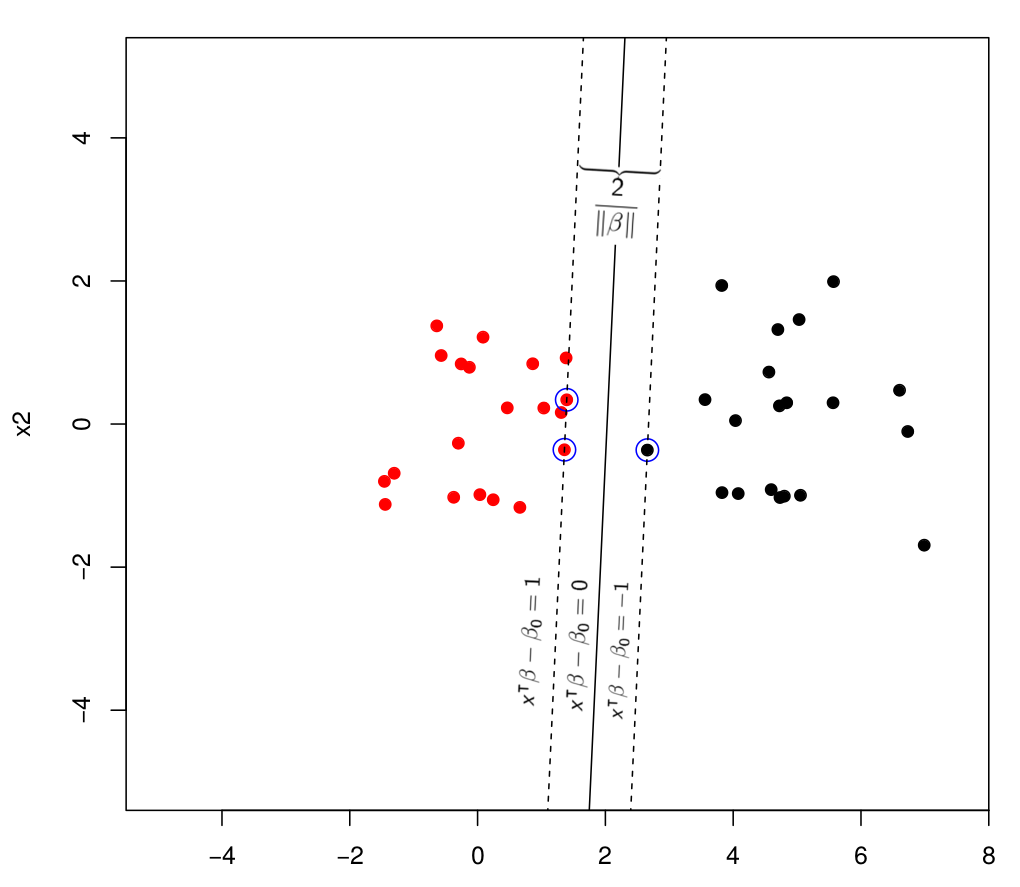
\includegraphics[width=0.7\textwidth]{plot.png}
	\end{figure}
\end{frame}

\begin{frame}{Hard-margin SVM}
	Предположим, что данные -- разделимы гиперплоскостью $x^\intercal \beta - \beta_0 = 0; \beta\in\mathbb{R}^p, \beta\in\mathbb{R}$.

	Определив расстояние со знаком $g\left(x\right)=x^\intercal \beta - \beta_0$,
можно считать, что $h\left(x_i\right)=\sign\left[g\left(x\right)\right]$.

	Из интуитивных соображений разумно полагать, что наилучшая разделяющая гиперплоскость -- та, которая
расположена дальше всего от представителей каждого из классов.

    $\frac{2}{\norm{\beta}}$ --- растояние между парой гиперплоскостей, симметричных относительно разделяющей, таких, что
    никакая из точек не лежит между ними --- называется отступом (margin).

	$$
	\begin{cases}
		\frac{1}{2}\norm{\beta}_2^2\rightarrow \min\limits_{\beta,\beta_0} \\
		y_i\left(x_i^\intercal \beta - \beta_0\right) \geq 1 \\
	\end{cases}
	$$
\end{frame}
\begin{frame}{Hard-margin SVM: множители Лагранжа}
	Воспользуемся методом множителей Лагранжа
	$$
	\begin{cases}
		\inf\limits_{\beta,\beta_0} \frac{1}{2}\norm{\beta}_2^2 - \sum\limits_{i=1}^n\alpha_i\left[y_i\left(x_i^\intercal\beta + \beta_0\right)-1\right] \rightarrow \max\limits_{\alpha_i} \\
		\alpha_i \geq 0, \forall i \\
		y_i\left(x_i^\intercal \beta - \beta_0\right) \geq 1 \\
	\end{cases}
	$$

	Так как оптимизируемая функция гладкая, можно воспользоваться необходимыми условиями экстремума

	$$
\begin{ecases}
\frac{\partial}{\partial \beta}: & \beta = \sum\limits_{i=1}^{n}\alpha_i y_i x_i \\
\frac{\partial}{\partial \beta_0}: & 0=\sum\limits_{i=1}^{n}\alpha_i y_i \\
\end{ecases}
	$$
\end{frame}
\begin{frame}{Hard-margin SVM: двойственная задача Вольфа}
	Двойственная задача Вольфа:
	\only<1>{
		$$
	\begin{cases}
		\frac{1}{2}\norm{\beta}_2^2 - \sum\limits_{i=1}^n\alpha_i\left[y_i\left(x_i^\intercal\beta + \beta_0\right)-1\right] \rightarrow \max\limits_{\alpha_i} \\
		\alpha_i \geq 0, \forall i \\
		\beta = \sum\limits_{i=1}^{n}\alpha_i y_i x_i \\
		0=\sum\limits_{i=1}^{n}\alpha_i y_i \\		
		y_i\left(x_i^\intercal \beta - \beta_0\right) \geq 1 \\
	\end{cases}
	$$
	}
	\only<2>{
		$$
	\begin{cases}
		\sum\limits_{i=1}^n \alpha_i - \frac{1}{2}\sum\limits_{i=1}^n\sum\limits_{i=1}^{n}\alpha_i\alpha_jy_iy_jx_i^\intercal x_j \rightarrow \max\limits_{\alpha_i} \\
		\alpha_i \geq 0, \forall i \\
		y_i\left(x_i^\intercal \beta - \beta_0\right) \geq 1 \\
	\beta = \sum\limits_{i=1}^{n}\alpha_i y_i x_i \\
 	\end{cases}
	$$
	}
\end{frame}

\begin{frame}{Опорные вектора}
	В точке оптимума выполнены условия Каруша-Куна-Такера, в частности:
	$$ \alpha_i \left[1-y_i\left(x_i^\intercal \beta - \beta_0\right)\right] = 0\, \forall i$$

	Т.е. либо
	\begin{itemize}
		\item $\alpha_i=0 \Rightarrow y_i g\left(x_i\right) > 1$ -- т.е. наблюдение не влияет на $\beta,\beta_0$
		\item $\alpha_i>0 \Rightarrow y_i g\left(x_i\right) = 1$ -- такое наблюдение будем называть опорным вектором
	\end{itemize}
	
	Из этих же соображений можно вычислить $\beta_0$ воспользовавшись произвольным опорным вектором.
\end{frame}

\subsection{Общий случай}
\begin{frame}{Slack variables}
	Обобщим процедуру на линейно-неразделимые данные

	Позволим каждому из ограничений быть нарушеным на $\xi_i$:
	$$y_i\left(x_i^\intercal \beta - \beta_0\right) \geq 1 - \xi_i, \xi_i \geq 0$$
	ограничив при этом суммарную ошибку некоторым параметром 
	$$\sum\limits_{i=1}^n \xi_i \leq t$$

	Можно отметить, что
	\begin{itemize}
		\item $\xi_i = 0$ -- наблюдения, лежащие вне зазора между классами
		\item $\xi_i \in \left(0; 1\right)$ -- правильно классифицированные наблюдения, лежащие внутри зазора
		\item $\xi_i \geq 1$ -- некорректно классифицированное наблюдения
	\end{itemize}

\end{frame}

\begin{frame}{Прямая задача}
	Сформулируем оптимизационную задачу аналогично линейно-разделимому случаю:
	$$
	\begin{cases}
		\frac{1}{2}\norm{\beta}_2^2\rightarrow \min\limits_{\beta,\beta_0} \\
		y_i\left(x_i^\intercal \beta - \beta_0\right) \geq 1 - \xi_i \\
		\sum\limits_{i=1}^n\xi_i \leq t \\
		\xi_i\geq 0 \\
	\end{cases}
	$$

    Величина отступа (margin), равная $\frac{2}{\norm{\beta}}$ в данном случае определяет расстояние между парой гиперплоскостей, параллельных разделяющей,
внутри которой присутствует пенальти за корректную классификацию.

	Применяя те же соображения (использование множителей Лагранжа, двойственной задачи в форме Вольфа, условия Каруша-Куна-Такера), переходим к двойственной задаче.

\end{frame}

\begin{frame}{Двойственная задача}
	После необходимых преобразований, получается двойственная задача:
	$$
	\begin{cases}
		\sum\limits_{i=1}^{n}\alpha_i - \frac{1}{2}\sum\limits_{i=1}^n\sum\limits_{j=1}^n\alpha_i\alpha_jy_iy_jx_i^\intercal x_j \rightarrow \max\limits_{\alpha_i} \\
		\alpha_i\in\left[0; t\right] \\
		\text{KKT+Wolfe conditions} \\
	\end{cases}
	$$

	При этом, так же как и в линейно-разделимом случае
	$$ \beta = \sum_{i=1}^n \alpha_i y_i x_i $$
	где $\alpha_i=0$ для части наблюдений (в которых ограничение соблюдается строго)
\end{frame}

\begin{frame}{Влияние параметра $t$}
	\begin{figure}
		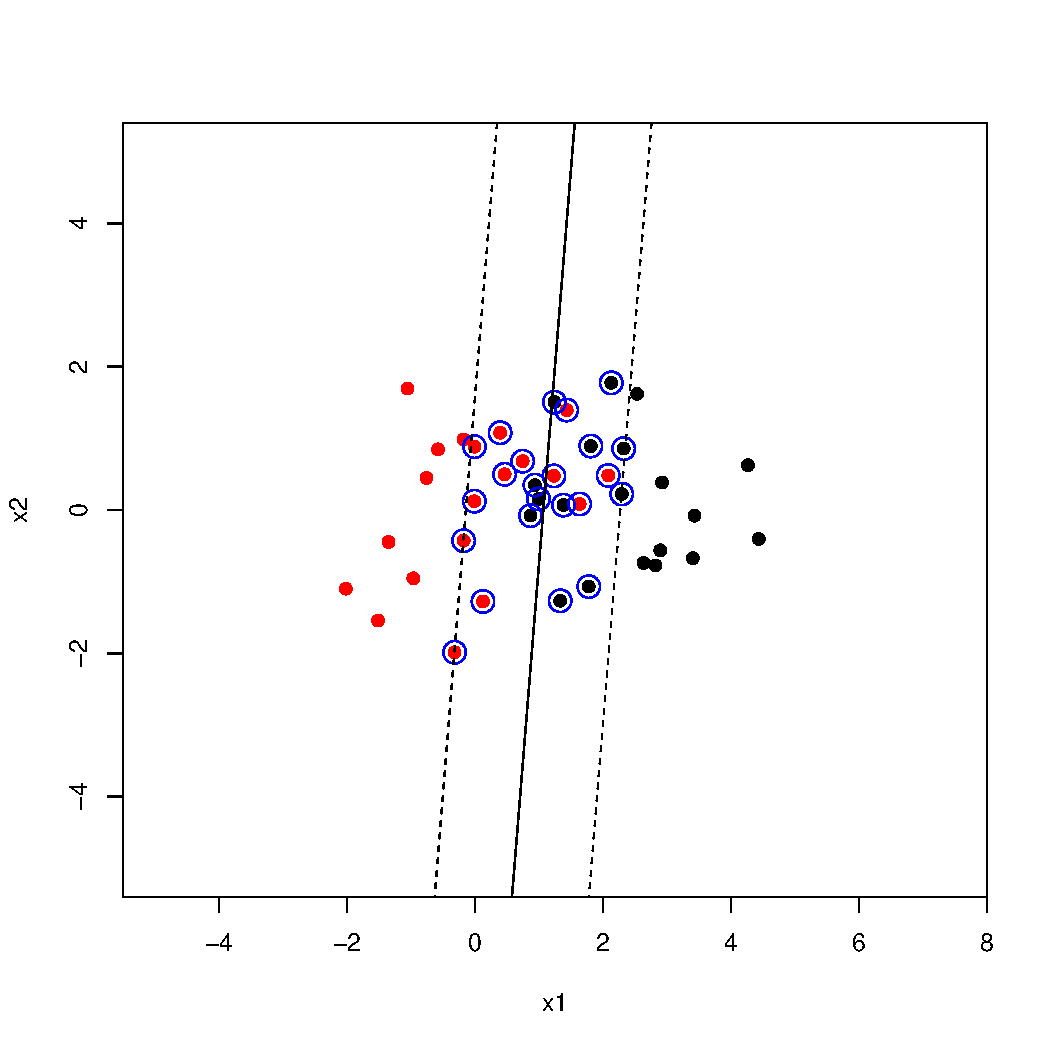
\includegraphics[width=0.5\textwidth]{plot1em2.pdf}%
		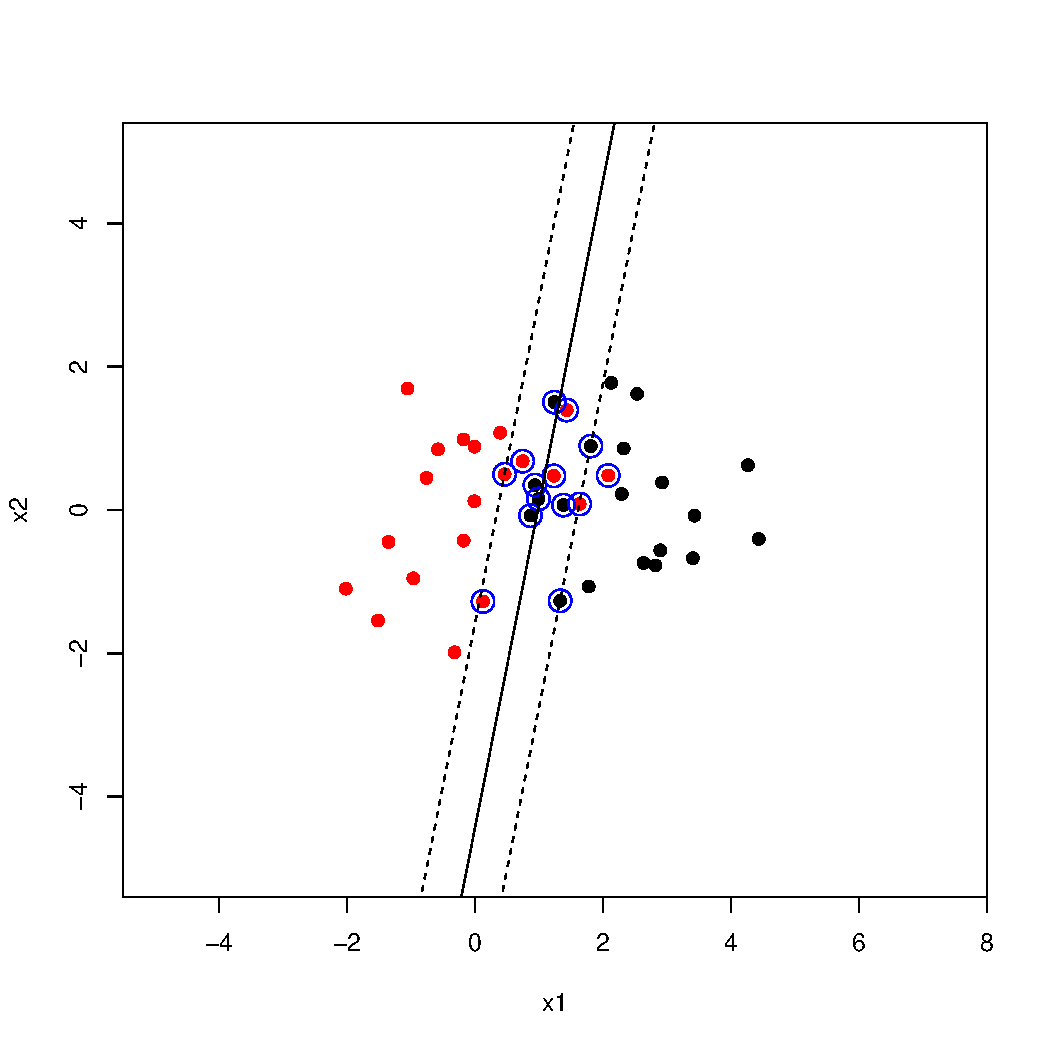
\includegraphics[width=0.5\textwidth]{plot1ep2.pdf}
		\caption{Влияние максимально допустимой ошибки на SVM}
	\end{figure}
\end{frame}

\subsection{SVM как Empirical Risk Minimization}
\begin{frame}{Эквивалентная переформулировка}
	Можно показать, что оптимизационная задача для soft-margin SVM эквивалентна задаче
	$$
		\sum\limits_{i=1}^n\max\left\{0, 1-y_i\left(x_i^\intercal \beta - \beta_0\right)\right\}+\eta\norm{\beta}^2_2\rightarrow \min\limits_{\beta,\beta_0}
	$$

	Таким образом, SVM можно рассматривать как минимизацию эмпирического риска (с регуляризацией $\eta\norm{\beta}_2^2$) и функцией потерь
	$$\max\left\{0, 1-y\left(x^\intercal \beta - \beta_0\right)\right\}$$

	Которую можно рассматривать, как непрерывную аппроксимацию разрывной ошибки классификации
	$$\mathbf{1}_{\left(h\left(x\right)\neq y\right)}$$
\end{frame}
\begin{frame}{Функция потерь в подходе Empirical Risk Minimization}
	\begin{columns}
		\begin{column}{0.5\textwidth}
			Функции потерь:
			\begin{itemize}
				\item Логистическая регрессия
					$ \log{1+e^{-g\left(x\right)y}}$
				\item SVM
					$ \max\left\{0, 1-g\left(x\right)y\right\}$
				\item Ошибка классификации: $ \mathbf{1}_{y\neq\sign{g\left(x\right)}} $
                \item LDA\footnote{В предположении одинаковых оценок $\hat{\pi}_i$}: $\left(1-g\left(x\right)\right)^2$
			\end{itemize}
		\end{column}
		\begin{column}{0.5\textwidth}
	\begin{figure}
		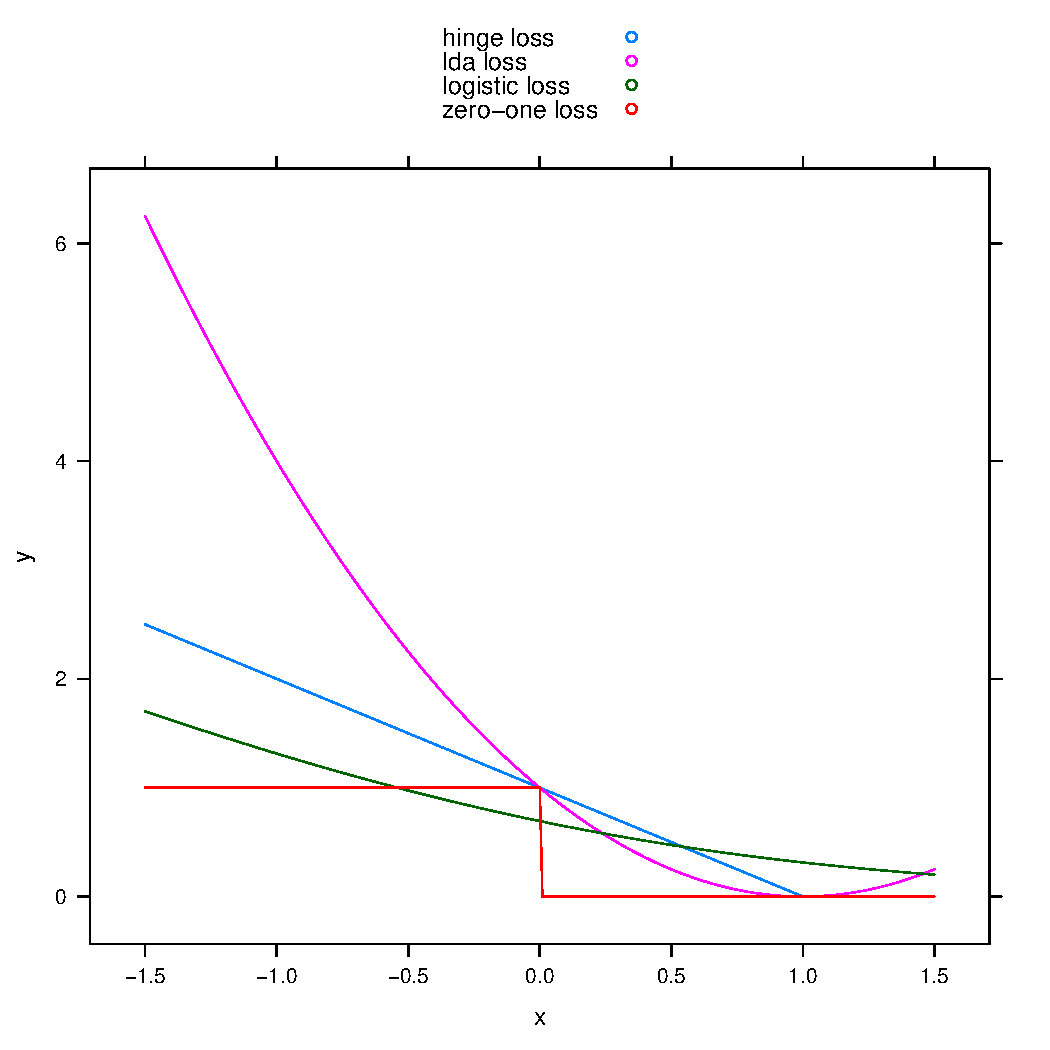
\includegraphics[width=1.0\textwidth]{loss.pdf}
	\end{figure}
		\end{column}
	\end{columns}
\end{frame}

\subsection{Алгоритмы оптимизации}
\begin{frame}{Методы поиска решений}
	Для soft-margin SVM нами были получены две эквивалентные задачи:
	\begin{itemize}
		\item Прямая задача ($d+1$ параметров, $O\left(n\right)$ ограничений):
			$$
	\begin{cases}
		\frac{1}{2}\norm{\beta}_2^2\rightarrow \min\limits_{\beta,\beta_0} \\
		\text{$O\left(n\right)$ ограничений неравенства}
	\end{cases}
			$$
		\item Двойственная задача ($n$ параметров, $O\left(n\right)$ ограничений):

			$$
	\begin{cases}
		\sum\limits_{i=1}^{n}\alpha_i - \frac{1}{2}\sum\limits_{i=1}^n\sum\limits_{j=1}^n\alpha_i\alpha_jy_iy_jx_i^\intercal x_j \rightarrow \max\limits_{\alpha_i} \\
		\text{$O\left(n\right)$ ограничений неравенства}
	\end{cases}
			$$
	\end{itemize}

	В зависимости от соотношения $d$ и $n$ разумно использовать прямую или двойственную задачу.
\end{frame}


\begin{frame}{Поиск решений прямой задачи}
	Пользуясь эквивалентной формулировкой прямой задачи
	$$
		\sum\limits_{i=1}^n\max\left\{0, 1-y_i\left(x_i^\intercal \beta - \beta_0\right)\right\}+\eta\norm{\beta}^2_2\rightarrow \min\limits_{\beta,\beta_0}
		$$

	Предлагается производить оптимизацию по $\beta$ используя стохастический градиентный спуск с аккуратным выбором величины шага.

	Можно показать\footnote[frame]{Pegasos: primal estimated sub-gradient solver
	for SVM}, что такой метод позволяет получить
решение с точностью $\varepsilon$ за $O\left(\frac{1}{\varepsilon}\right)$ итераций; при этом количество наблюдений не влияет на
    асимптотику количества итераций (но сложность одной итерации зависит от количества наблюдений).
\end{frame}

\begin{frame}{Поиск решений двойственной задачи}
	Для двойственной задачи 
	$$
		\mathcal{F}\left(\alpha_1,\dots,\alpha_n\right) = \sum\limits_{i=1}^{n}\alpha_i - \frac{1}{2}\sum\limits_{i=1}^n\sum\limits_{j=1}^n\alpha_i\alpha_jy_iy_jx_i^\intercal x_j \rightarrow \max\limits_{\alpha_i}
	$$

	Предлагается\footnote[frame]{A Dual Coordinate Descent Method for Large-scale Linear SVM} совершить несколько итераций покоординатного градиентного спуска:
	\begin{itemize}
		\item Каждый $\alpha_i$ изменяется в направлении $\frac{\partial \mathcal{F}}{\partial \alpha_i}$
		\item Очередное решение проецируется на множество допустимых
		\item Поддерживается необходимая для вычисления $x^\intercal \beta$ информация
	\end{itemize}

	Последовательность решений сходится как минимум линейно

\end{frame}

\section{Расширения SVM}
\subsection{Kernel trick}
\begin{frame}{Спрямляющее пространство}
	По построению, SVM применим лишь к (почти) линейно-разделимым данным.

	Предположим, что известен набор отображений 
	$$\left\{\varphi_j\left(x\right)\right\}_{j=1}^{d}$$
	$$\varphi_j:\mathbb{R}^p\rightarrow \mathbb{R}$$
	таких, что набор данных 
	$$\left\{\tilde{x}_i=\begin{pmatrix}
		\varphi_1\left(x_i\right) \\
		\vdots \\
		\varphi_d\left(x_i\right) \\
	\end{pmatrix}, y_i\right\}_{i=1}^{n}$$
	линейно разделим; будем называть пространство, в котором наблюдается
	разделимость, спрямляющим пространством
	
\end{frame}

\begin{frame}{Двойственная задача в спрямляющем пространстве}
	Записывая двойственную задачу в спрямляющем пространстве,
	$$
		\sum\limits_{i=1}^{n}\alpha_i - \frac{1}{2}\sum\limits_{i=1}^n\sum\limits_{j=1}^n\alpha_i\alpha_jy_iy_j\tilde{x}_i^\intercal \tilde{x}_j \rightarrow \max\limits_{\alpha_i} 
	$$
	можно заметить, что $\tilde{x}_i$ входят в её формулировку лишь в виде скалярных произведений $\tilde{x}_i^\intercal \tilde{x}_j$.

	Также, используя выражение
	$$\beta = \sum\limits_{i=1}^{n}\alpha_i y_i \tilde{x}_i$$
	вычисление расстояния до разделяющей гиперплоскости (со знаком)
	также сводится к использованию скалярных произведений $\tilde{x}_i$.

\end{frame}

\begin{frame}{Kernel-trick: Теорема Мерсера}
	Таким образом, скалярного произведения в спрямляющем
	пространстве достаточно для построения (и применения) классифицирующего правила.

	Кроме того, знание отображений $\varphi_j$ не требуется и спрямляющее пространство может быть бесконечномерным.
\end{frame}

\begin{frame}{Kernel-trick: Теорема Мерсера}

	\begin{thr}
		Пусть $K\left(u,v\right):X\times X\rightarrow \mathbb{R}$ -- отображение:
		\begin{itemize}
			\item Симметричное: $K\left(u, v\right)=K\left(v, u\right)$
			\item Положительно определённое: $\iint\limits_{X\times X}K\left(u,v\right)g\left(u\right)g\left(v\right)\diff{u}\diff{v}\geq 0, \forall g:X\rightarrow \mathbb{R}$
		\end{itemize}

		Тогда (и только тогда) существует пространство $H$ и отображение $\varphi:X\rightarrow H: K\left(u, v\right)=\left\langle\varphi\left(u\right), \varphi\left(v\right)\right\rangle_H$
	\end{thr}

	Таким образом, для любой функции, являющейся ядром, существует пространство со
	скалярным произведением.
    
    Цель использования данного соображения применительно к SVM в том, что после перехода в новое пространство
    (с помощью $\varphi$)  исходные данные могут стать почти линейно-разделимыми.
\end{frame}

\begin{frame}{Kernel-trick: операции над ядрами}
	Известны некоторые способы конструирования ядер, позволяющие не проверять условия теоремы Мерсера:
	\begin{itemize}
		\item Скалярное произведение в векторном пространстве
		\item Положительная константа
		\item Произведение ядер: $K\left(u,v\right)=K_1\left(u,v\right)K_2\left(u, v\right)$
		\item Произведение отображений: $K\left(u, v\right)=\varphi\left(u\right)\varphi\left(v\right), \varphi:X\rightarrow \mathbb{R}$
		\item Линейная комбинация с положительными коэффициентами: $K\left(u, v\right)=\alpha_1K_1\left(u,v\right)+\alpha_2K_2\left(u, v\right), \alpha_{1,2}>0$
		\item Композиция ядра и отображения: $K\left(u, v\right)=K_1\left(\varphi\left(u\right),\varphi\left(v\right)\right)$
		\item Степенной ряд: 
			$$f: \mathbb{R}\rightarrow\mathbb{R}$$
			сходящийся степенной ряд с положительными коэффициентами, тогда
			$$K\left(u, v\right)=f\left(K_1\left(u,v\right)\right)$$
			является ядром
	\end{itemize}
\end{frame}

\begin{frame}{Kernel-trick: примеры ядер}
	Используя предыдущие рассуждения, несложно показать, что ядрами являются:
	\begin{itemize}
		\item Полиномиальное ядро: $K\left(u,v\right)=\left(1+\left\langle u, v\right\rangle\right)^d$ (базисные функции -- мономы степени $\leq d$; размерность пространства -- $C_{p+d}^d$
		\item Ядро радиальных базисных функций: $K\left(u, v\right)=e^{-\frac{\norm{u-v}^2_2}{2\sigma^2}}$
	\end{itemize}

    Выбор ядра может быть обусловлен либо знанием о данных (например эмпирическим, в случае если они похожи на отделимые поверхностями соответствующего порядка),
    либо производится автоматически на основе кросс-валидации или иной процедуры
\end{frame}

\subsection{Multi-class SVM}
\begin{frame}{Множественная классификация: one vs one}
	Построение SVM происходило для классификации с двумя классами; покажем, как можно
	обобщить полученное решение на классификацию с $N$ классами:

	\begin{itemize}
		\item Для всех $\frac{N\left(N + 1\right)}{2}$ пар классов построим SVM-классификатор
		\item Обозначим за $N_i\left(x\right)$ количество парных классификаций, в которых был выбран класс $i$
	\end{itemize}

	Классифицирующее правило: $g\left(x\right)=\argmax\limits_i N_i\left(x\right)$
\end{frame}

\begin{frame}{Множественная классификация: one vs other}
	Покажем иное построение классификации с $N$ классами, использующее меньшее
	количество классификаторов.

	\begin{itemize}
		\item Построим $N$ классификаторов для задач классификации 
			$$y_i=1\Leftrightarrow x_i\text{ из $i$-го класса}$$
		\item
			Соответствующее классифицирующее правило обозначим 
			$$ g_i\left(x\right) = \sign\left(h_i\left(x\right)\right))$$
	\end{itemize}

	Классифицирующее правило: $g\left(x\right)=\argmax\limits_i h_i\left(x\right)$
\end{frame}

\subsection{SVM regression}
\begin{frame}{Регрессия с помощью SVM}
	Сформулируем задачу регрессии в виде, похожем на SVM:
	$$
	\begin{cases}
		C\sum\limits_{i=1}^n\left(\xi_i^{+}+\xi_i^{-}\right) +\frac{1}{2}\norm{\beta}^2_2\rightarrow \min\limits_{\beta,\beta_0} \\
		\xi_i^{+}, \xi_i^{-} \geq 0 \\
		y_i - \left(x_i^\intercal \beta + \beta_0\right) \leq \varepsilon + \xi_i^{+} \\
		-y_i + \left(x_i^\intercal \beta + \beta_0\right) \leq \varepsilon + \xi_i^{-} \\
	\end{cases}
	$$

	Оказывается, что в такой формулировке
	\begin{itemize}
		\item $\beta$ описывается как линейная комбинация опорных векторов
		\item В двойственной задаче $x_i$ встречаются только в виде скалярных произведений $\Rightarrow$ можно использовать kernel-trick
	\end{itemize}

\end{frame}

\subsection{Изменение регуляризации}
\begin{frame}{Изменение регуляризации в SVM}
	С целью отбора признаков можно изменить регуляризацию в одной из
	эквивалентных формулировок SVM:

	$$
		C\sum\limits_{i=1}^n\max\left\{0, 1-y_i\left(x_i^\intercal \beta - \beta_0\right)\right\}+\Phi\left(\beta\right)\rightarrow \min\limits_{\beta,\beta_0}
	$$

	\begin{itemize}
		\item LASSO SVM: $\Phi\left(\beta\right)=\norm{\beta}_1$
		\item Doubly-regularized SVM: $\Phi\left(\beta\right)=\alpha\norm{\beta}_1+\frac{1}{2}\norm{\beta}_2^2$
		\item Support Features Machine: $\Phi\left(\beta\right)=\sum\limits_{i=1}^{p}\max\left\{2\mu\beta_i, \mu^2+\beta_i^2\right\}$
		\item Relevance Features Machine: $\Phi\left(\beta\right)=\sum\limits_{i=1}^{p}\ln\left(\beta_i^2+\frac{1}{\mu}\right)$
	\end{itemize}

    ($\alpha, \mu$ --- дополнительные параметры; коэффициент soft-margin SVM $t$, эквивалентным преобразованием перемещён к $\sum$)
\end{frame}

\section{Выбор параметров}
\subsection{Кросс-валидация}
\begin{frame}{Выбор параметров с помощью кросс-валидации}
	SVM требует выбора максимально возможного нарушения
	ограничений $t$, в случае использования kernel-trick --- выбора ядра и, возможно,
	параметров ядра; а также --- параметров регуляризатора в SVM-подобных процедурах.


	Для выбора оптимального набора параметров предлагается воспользоваться кросс-валидацией:
	\begin{itemize}
		\item Данные разделяются на $K$ частей сходного размера
		\item Для всех $k=1,\dots,K$ строится оценка $\hat{\beta}^{(k)},\hat{\beta}_0^{(k)}$
			по данным из всех частей, кроме $k$-ой
		\item Для всех $k$ по отброшенной части данных строится оценка ошибочной классификации:
			$ \varepsilon_k = \frac{n_k}{n}\mathbf{1}_{y_i\neq y_i^{(k)}} $
		\item Строится оценка качества классификации $\mathcal{E}=\sum\limits_k \varepsilon_k$
	\end{itemize}

	Из всего рассматриваемого пространства параметров выбирается набор параметров,
	минимизирующих $\mathcal{E}$; после чего с использованием этого набора параметров
	строится модель по всем данным.
\end{frame}

\begin{frame}{Некоторые соображения о кросс-валидации}
	Терминология:
	\begin{itemize}
		\item K-fold cross-validation -- кросс-валидация с разделением на $K$ частей
		\item Leave-one-out cross-validation -- кросс-валидация с разделением на одноэлементные множества
	\end{itemize}

	Полезные соображения:
	\begin{itemize}
	
	\item Соображения кросс-валидации применимы и к регрессии, в этом случае может использоваться
	оценка
	$$\varepsilon_k=\frac{n_k}{n}\text{MSE}_k$$

    \item Важно применять кросс-валидацию ко всей процедуре оценки параметров в целом, не допуская
   использования всех доступных данных на каком-либо промежуточном этапе
    \item Оценка качества классификации (MSE регрессии) получается смещённой (с положительным смещением),
        так как оценка параметров производится по меньшим наборам данных
	\end{itemize}
\end{frame}

\subsection{Комбинаторная размерность}
\begin{frame}
	В рамках SVM можно предъявить оценку, связывающую математическое ожидание
ошибки классификации и эмпирическую ошибку классификации.

	Пусть $x_i,y$ -- выборка из распределения $P\left(x, y\right)$, определим:
	\begin{itemize}
		\item $y=f\left(x,\alpha\right)$ -- модель классификатора, зависящая от $\alpha$
		\item Математическое ожидание ошибки классификации
			$$R\left(\alpha\right)=\int \mathbf{1}_{y\neq f\left(x, \alpha\right)}\diff{P\left(x,y\right)}$$
		\item Эмпирическая ошибка классификации
			$$R_e\left(\alpha\right)=\frac{1}{n}\sum_{i=1}^n \mathbf{1}_{y_i\neq f\left(x_i, \alpha\right)}$$
	\end{itemize}
\end{frame}

\begin{frame}
	При этом с вероятностью $1-\eta$, $0<\eta<1$ выполнено:
	$$	R\left(\alpha\right) \leq R_e\left(\alpha\right)+\sqrt{\frac{h\left(1+\log{\frac{2n}{h}}\right)-\log\frac{\eta}{4}}{n}}$$

	Где $h$ -- размерность Вапника-Червоненкиса (VC-размерность), характеризующая
	сложность семейства алгоритмов для классификации с двумя классами.
	\begin{itemize}
		\item Для гиперплоскостей в $\mathbb{R}^p$: $h=p+1$
		\item Если любой набор из $k$ точек разделим для любого назначения классов $\Rightarrow h\geq k$
        \item С помощью данного факта можно получить оценку сверху на математическое ожидание ошибки классификации
            для некоторых классов функций
        \item Легко видеть, что при $n\rightarrow\infty$ оценка сходится к $R_e$
	\end{itemize}
\end{frame}


\section{Сравнение с другими методами}
\begin{frame}{Сравнение SVM с LDA}
    \begin{minipage}{0.46\textwidth}
    Оптимизационная задача SVM:
    $$
	\begin{cases}
		\frac{1}{2}\norm{\beta}_2^2\rightarrow \min\limits_{\beta,\beta_0} \\
		y_i\left(x_i^\intercal \beta - \beta_0\right) \geq 1 - \xi_i \\
		\sum\limits_{i=1}^n\xi_i \leq t \\
		\xi_i\geq 0 \\
	\end{cases}
    $$
    \end{minipage}
    \begin{minipage}{0.46\textwidth}
    Оптимизационная задача LDA:
    $$
    \begin{cases}
    \beta^\intercal \Sigma_B \beta \rightarrow \max \\
    \beta^\intercal \Sigma_W \beta = 1\\
    \end{cases}
    $$
    \end{minipage}

    \begin{itemize}
        \item LDA (в построении) предполагает нормальность; SVM --- свободен от предположений
            о распределении данных
        \item На построение решающего правила при помощи LDA влияют все наблюдения,
            при использовании SVM -- только опорные вектора
        \item В LDA (в отличие от SVM) априрорные вероятности принадлежности классу влияют на сдвиг границы классификации
        \item LDA имеет аналитическое решение (с помощью обобщённых собственных векторов)
        \item Оба метода допускают использование kernel-trick
    \end{itemize}
\end{frame}


\end{document}


